%%%%%%%%%%%%%%%%%%%%%%%%%%%%%%%%%%%%%%%%%%%%%%%%%%%%%%%%%%%%%%%%%%%%%%%%%%%%%%%%%%
\begin{frame}[fragile]\frametitle{}
\begin{center}
{\Large Introduction}
\end{center}
\end{frame}


%%%%%%%%%%%%%%%%%%%%%%%%%%%%%%%%%%%%%%%%%%%%%%%%%%%%%%%%%%%%%%%%%%%%%%%%%%%%%%%%%%
\begin{frame}[fragile]\frametitle{Introduction to Yoganidra}
	\begin{itemize}
		\item \textbf{Yoga Nidra (योगनिद्रा)} is a deep relaxation technique that:
			\begin{itemize}
				\item Relieves stress.
				\item Improves sleep.
				\item Accesses the bliss state (Ananda आनन्द).
			\end{itemize}
	\item Composed of series of body, breath, imagination acts to guide into progressive states of relaxation (non-doing)
    \item \textbf{Inspired by the Bihar School of Yoga}, this script follows the inward journey through the Koshas.
	\end{itemize}
	
\end{frame}

%%%%%%%%%%%%%%%%%%%%%%%%%%%%%%%%%%%%%%%%%%%%%%%%%%%%%%%%%%%%%%%%%%%%%%%%%%%%%%%%%%
\begin{frame}[fragile]\frametitle{Introduction to Yoganidra}
    \begin{itemize}
        \item \textbf{Yoganidra} translates to "yogic sleep" and represents a state of deep relaxation.
        \item Often referred to as the "4th state" or \textbf{Turya} in Mandukya Upanishad.
        \item Unlike regular sleep, Yoganidra involves deep relaxation combined with heightened awareness.
        \item Practiced through guided meditations that induce states of restful alertness.
    \end{itemize}
\end{frame}

%%%%%%%%%%%%%%%%%%%%%%%%%%%%%%%%%%%%%%%%%%%%%%%%%%%%%%%%%%%%%%%%%%%%%%%%%%%%%%%%%%
\begin{frame}[fragile]\frametitle{Borderline between Awake and Sleep}
    \begin{itemize}
        \item Yoganidra is on the borderline between wakefulness and sleep.
        \item It balances conscious and subconscious awareness, bridging the gap between these states.
        \item Practitioners bypass the usual conscious filtering, allowing direct access to the subconscious.
    \end{itemize}
\end{frame}

%%%%%%%%%%%%%%%%%%%%%%%%%%%%%%%%%%%%%%%%%%%%%%%%%%%%%%%%%%%
\begin{frame}[fragile]\frametitle{What is Yoga Nidra?}
      \begin{center}
        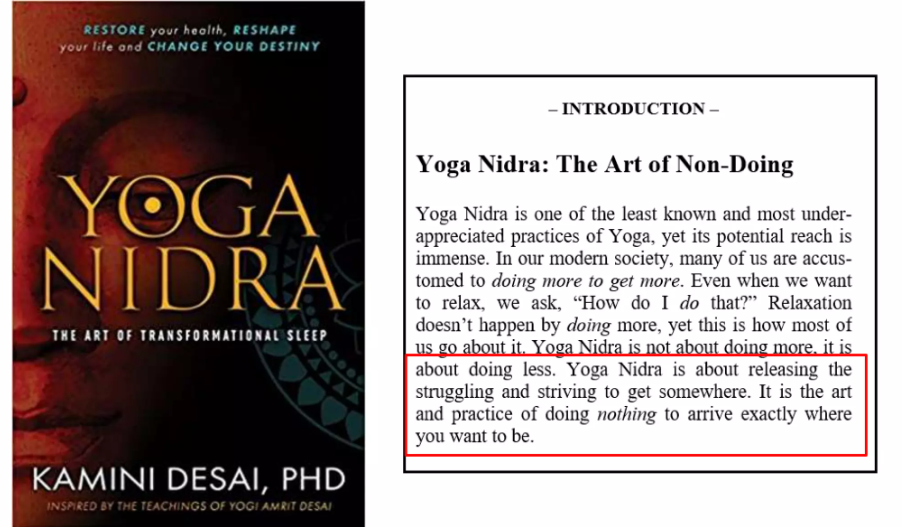
\includegraphics[width=\linewidth,keepaspectratio]{yoganidra1}

		{\tiny (Ref: Yoga Nidra - Dr Amit Chail)}		
        \end{center}

\end{frame}

%%%%%%%%%%%%%%%%%%%%%%%%%%%%%%%%%%%%%%%%%%%%%%%%%%%%%%%%%%%
\begin{frame}[fragile]\frametitle{What is Yoga Nidra?}
Its is Pratyahara प्रत्याहार  : Prati प्रति (inside) + ahara आहार  (food), ie food to inside, that is, contrary to our attention being always external looking, here we are looking inside. Plus, there is tantra word 'nyasa' न्यास , meanings seating. meaning you put attention at different places.

      \begin{center}
        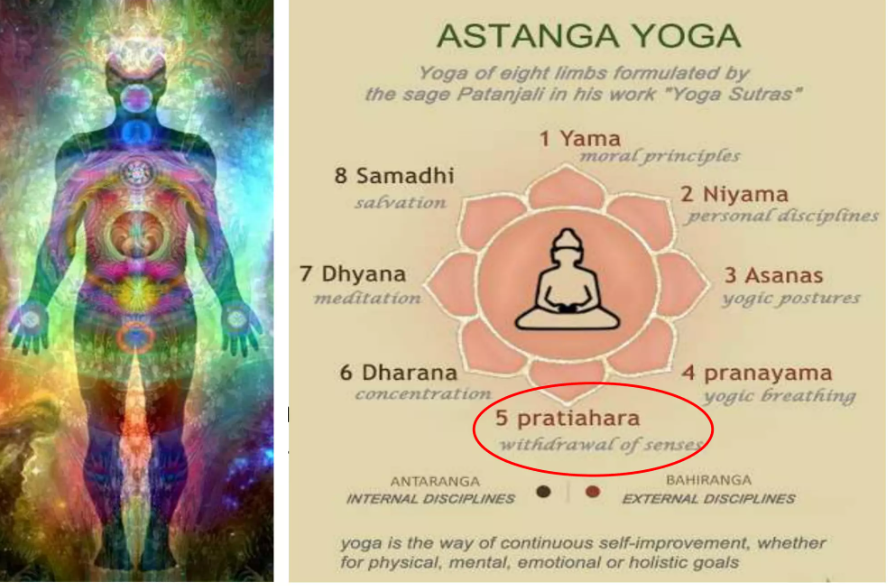
\includegraphics[width=0.6\linewidth,keepaspectratio]{yoganidra2}

		{\tiny (Ref: Yoga Nidra - Dr Amit Chail)}		
        \end{center}

\end{frame}

%%%%%%%%%%%%%%%%%%%%%%%%%%%%%%%%%%%%%%%%%%%%%%%%%%%%%%%%%%%
\begin{frame}[fragile]\frametitle{History}
      \begin{center}
        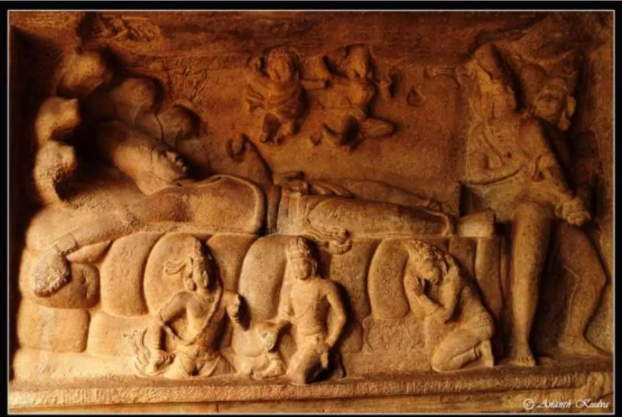
\includegraphics[width=0.8\linewidth,keepaspectratio]{yoganidra3}

		{\tiny (Ref: Yoga Nidra - Dr Amit Chail)}		
        \end{center}

\end{frame}

%%%%%%%%%%%%%%%%%%%%%%%%%%%%%%%%%%%%%%%%%%%%%%%%%%%%%%%%%%%%%%%%%%%%%%%%%%%%%%%%%%
\begin{frame}[fragile]\frametitle{Notable points}
    \begin{itemize}
        \item Yoganidra comes from tantra तंत्र  , where it is called 'nyasa' न्यास (withdraw, like Pratyahara प्रत्याहार), meaning withdraw from acquired self full of anxiety and worry, and go inward to become real self who is calm and peaceful.
		\item Yoganidra works on manas मनस  (which is feminine, motherly) and not on buddhi बुद्धी(which is masculine, fatherly)
		\item Swami Satyanand Sawarswati revived it after loss in centuries in between, now given to Swammi Niranjanananda.
		\item Yogasutra is part of 6 darshana दर्शन(yoga योग), which is 'what' and 'how' process, tantra and not just 'what' in case of word 'Philosophy', purely theoretical.
		\item Bhagavad geeta भगवदगीता  starts with word 'dharma kshetre' धर्मक्षेत्रे   so its about 'dharma' धर्म.    Yogasutra starts with word 'atha yoga anushasanam' अथ  योग अनुशासनं, so, 'atha' अथ means 'now. Its all about 'now' the awareness of the present, that's it.
		\item The world will not adjust to your needs, you accept and withdraw to do your work.
    \end{itemize}
	
	{\tiny (Ref: Yoga Nidra (online) - Shrimath Yoga)}

\end{frame}

%%%%%%%%%%%%%%%%%%%%%%%%%%%%%%%%%%%%%%%%%%%%%%%%%%%%%%%%%%%%%%%%%%%%%%%%%%%%%%%%%%
\begin{frame}[fragile]\frametitle{Notable points}
    \begin{itemize}
        \item Make list of desires however small, keep them secret, will turn one of them to resolve.
		\item Mind has 4 modes: manas buddhi chitta ahamkar मनस बुद्धी चित्त अहंकार , we need to regulate it. one mode is active predominantly.
		\item manas: when ideating, brain-storming, when no judgment is exercised
		\item buddhi: selection of ideas/alternatives, using intellect filter whats needed
		\item chitta: memory, go to past, whats the experience of past (hard-disk)
		\item ahamkara: ego/self-arrogating(assignment)-principle is attached, is it suitable to me. To have will power to implement decisions taken.
    \end{itemize}
	
	{\tiny (Ref: Yoga Nidra (online) - Shrimath Yoga)}

\end{frame}


%%%%%%%%%%%%%%%%%%%%%%%%%%%%%%%%%%%%%%%%%%%%%%%%%%%%%%%%%%%
\begin{frame}[fragile]\frametitle{Four Stages of Human Consciousness}
      \begin{center}
        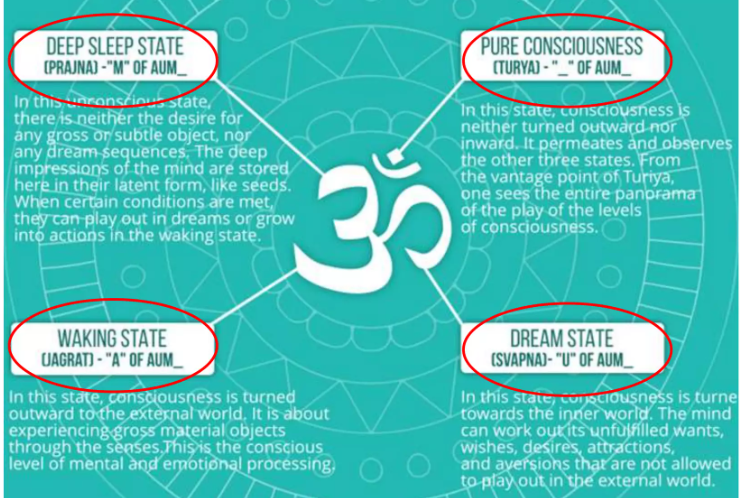
\includegraphics[width=0.8\linewidth,keepaspectratio]{yoganidra4}

		{\tiny (Ref: Yoga Nidra - Dr Amit Chail)}		
        \end{center}

\end{frame}

%%%%%%%%%%%%%%%%%%%%%%%%%%%%%%%%%%%%%%%%%%%%%%%%%%%%%%%%%%%
\begin{frame}[fragile]\frametitle{Brain Wave States in Yoga Nidra}
    \begin{itemize}
        \item During Yoga Nidra, consciousness fluctuates between:
        \begin{itemize}
            \item Introversion and extroversion states
            \item Alpha and theta wave states
        \end{itemize}
        \item \textbf{The Nidra State:}
        \begin{itemize}
            \item Located at border between alpha and theta waves
            \item Mind becomes highly receptive
            \item Allows contact with subconscious and unconscious dimensions
            \item Access to dormant potential and hidden solutions
        \end{itemize}
    \end{itemize}
\end{frame}

%%%%%%%%%%%%%%%%%%%%%%%%%%%%%%%%%%%%%%%%%%%%%%%%%%%%%%%%%%%%%%%%%%%%%%%%%%%%%%%%%%
\begin{frame}[fragile]\frametitle{Scientific Evidence of Brain States}
    \begin{itemize}
        \item \textbf{Alpha Brainwaves:}
        \begin{itemize}
            \item Associated with relaxation and creativity
            \item Enhanced learning capabilities
            \item Improved cognitive function
        \end{itemize}
        \item \textbf{Brain Coherence:}
        \begin{itemize}
            \item Different regions synchronize activity
            \item Similar to experienced meditators
            \item Access to deeper consciousness states
        \end{itemize}
        \item \textbf{Autonomic Nervous System:}
        \begin{itemize}
            \item Activates parasympathetic response
            \item Reduces effects of chronic stress
            \item Promotes natural healing processes
        \end{itemize}
    \end{itemize}
\end{frame}

%%%%%%%%%%%%%%%%%%%%%%%%%%%%%%%%%%%%%%%%%%%%%%%%%%%%%%%%%%%
\begin{frame}[fragile]\frametitle{Practitioners}
      \begin{center}
        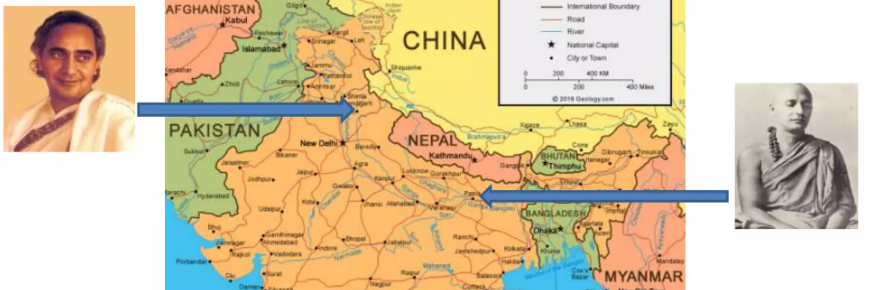
\includegraphics[width=\linewidth,keepaspectratio]{yoganidra5}

		{\tiny (Ref: Yoga Nidra - Dr Amit Chail)}		
        \end{center}

\end{frame}

%%%%%%%%%%%%%%%%%%%%%%%%%%%%%%%%%%%%%%%%%%%%%%%%%%%%%%%%%%%
\begin{frame}[fragile]\frametitle{Modern Development}
    \textbf{Swami Satyananda Saraswati's Contributions:}
    \begin{itemize}
        \item Systematized Yoga Nidra in the 20th century
        \item Founded Bihar School of Yoga
        \item Made the practice accessible to modern practitioners
        \item Emphasized scientific approach to traditional practice
        \item Developed structured methodology for teaching
    \end{itemize}
\end{frame}

%%%%%%%%%%%%%%%%%%%%%%%%%%%%%%%%%%%%%%%%%%%%%%%%%%%%%%%%%%%
\begin{frame}[fragile]\frametitle{Research}
      \begin{center}
        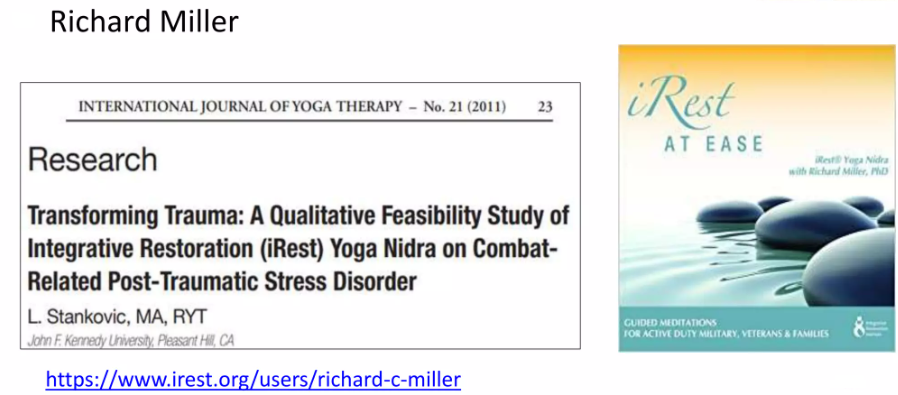
\includegraphics[width=\linewidth,keepaspectratio]{yoganidra6}

		{\tiny (Ref: Yoga Nidra - Dr Amit Chail)}		
        \end{center}

\end{frame}

%%%%%%%%%%%%%%%%%%%%%%%%%%%%%%%%%%%%%%%%%%%%%%%%%%%%%%%%%%%%%%%%%%%%%%%%%%%%%%%%%%
\begin{frame}[fragile]\frametitle{Sleep vs Yoga Nidra}
    \begin{columns}
        \begin{column}{0.48\textwidth}
            \textbf{Sleep:}
            \begin{itemize}
                \item Unconscious state
                \item No awareness
                \item Natural occurrence
                \item Brain in delta waves
            \end{itemize}
        \end{column}
        \begin{column}{0.48\textwidth}
            \textbf{Yoga Nidra (योगनिद्रा):}
            \begin{itemize}
                \item Conscious relaxation
                \item Maintained awareness
                \item Guided practice
                \item Brain transitions through various wave states
                \item One hour equals 4 hours of regular sleep
            \end{itemize}
        \end{column}
    \end{columns}
\end{frame}

% %%%%%%%%%%%%%%%%%%%%%%%%%%%%%%%%%%%%%%%%%%%%%%%%%%%%%%%%%%%%%%%%%%%%%%%%%%%%%%%%%%
% \begin{frame}[fragile]\frametitle{Nidra vs Yoganidra}
    % \textbf{Nidra (निद्रा)}: \\
    % \begin{itemize}
        % \item Unaware, only physical relaxation.
        % \item Unconscious state.
    % \end{itemize}
    % \vspace{5mm}
    % \textbf{Yoganidra (योगनिद्रा)}: \\
    % \begin{itemize}
        % \item Aware relaxation (physical, mental, and emotional).
        % \item Conscious of subconscious mind.
    % \end{itemize}
% \end{frame}

%%%%%%%%%%%%%%%%%%%%%%%%%%%%%%%%%%%%%%%%%%%%%%%%%%%%%%%%%%%%%%%%%%%%%%%%%%%%%%%%%%
\begin{frame}[fragile]\frametitle{Meditation vs Yoganidra}
    \begin{columns}
        \begin{column}{0.48\textwidth}
            \textbf{Meditation:}
            \begin{itemize}
                \item Typically done sitting up
                \item Focuses on one point of concentration
                \item Requires active mental effort
                \item May be challenging for beginners
            \end{itemize}
        \end{column}
        \begin{column}{0.48\textwidth}
            \textbf{Yoga Nidra (योगनिद्रा):}
            \begin{itemize}
                \item Done lying down
                \item Systematic rotation of awareness
                \item Guided relaxation practice
                \item Accessible to all skill levels
            \end{itemize}
        \end{column}
    \end{columns}
\end{frame}

%%%%%%%%%%%%%%%%%%%%%%%%%%%%%%%%%%%%%%%%%%%%%%%%%%%%%%%%%%%%%%%%%%%%%%%%%%%%%%%%%%
\begin{frame}[fragile]\frametitle{Differences between Yoganidra and Self-Hypnosis}
    \begin{itemize}
        \item \textbf{State of Consciousness:}
            \begin{itemize}
                \item \textbf{Yoganidra:} Achieves a state of Turya – deep relaxation with heightened awareness; mind remains alert.
                \item \textbf{Self-Hypnosis:} Involves a trance-like state where the conscious mind becomes passive, with a focus on specific suggestions.
            \end{itemize}
        \item \textbf{Process:}
            \begin{itemize}
                \item \textbf{Yoganidra:} Uses guided meditation to systematically relax each body part while retaining self-awareness.
                \item \textbf{Self-Hypnosis:} Often uses repetitive suggestions or imagery to access the subconscious for specific goals.
            \end{itemize}
        \item \textbf{Purpose:}
            \begin{itemize}
                \item \textbf{Yoganidra:} Aims for overall relaxation, self-awareness, and mental clarity; spiritual alignment.
                \item \textbf{Self-Hypnosis:} Typically used for behavior modification or addressing specific habits.
            \end{itemize}
        \item \textbf{Awareness Levels:}
            \begin{itemize}
                \item \textbf{Yoganidra:} Maintains a balance between conscious and subconscious, with an element of witnessing.
                \item \textbf{Self-Hypnosis:} Primarily engages the subconscious with reduced conscious interference.
            \end{itemize}
        \item \textbf{Applications:}
            \begin{itemize}
                \item \textbf{Yoganidra:} Stress reduction, relaxation, self-exploration, and spiritual growth.
                \item \textbf{Self-Hypnosis:} Often goal-oriented, targeting specific habits like smoking cessation, or reducing anxiety.
            \end{itemize}
    \end{itemize}
\end{frame}


%%%%%%%%%%%%%%%%%%%%%%%%%%%%%%%%%%%%%%%%%%%%%%%%%%%%%%%%%%%
\begin{frame}[fragile]\frametitle{Science: ECG}
      \begin{center}
        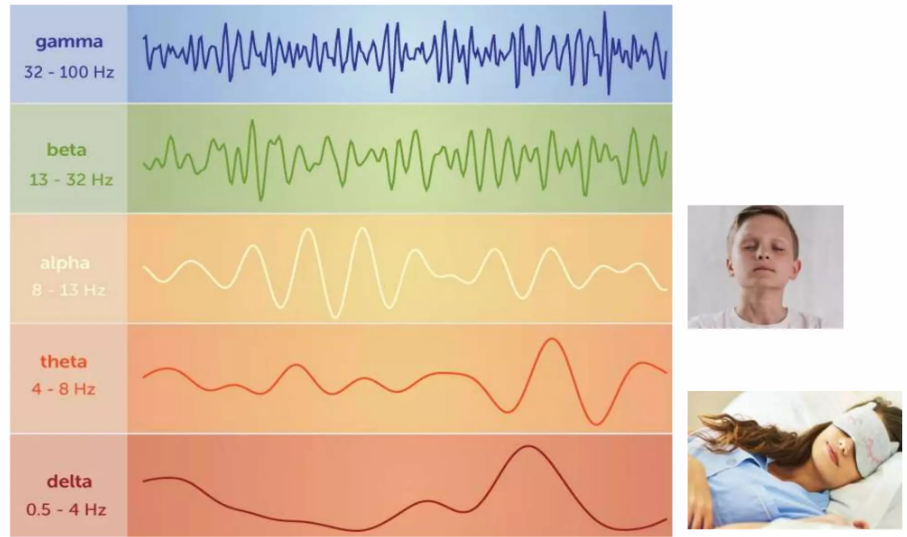
\includegraphics[width=\linewidth,keepaspectratio]{yoganidra9}

		{\tiny (Ref: Yoga Nidra - Dr Amit Chail)}		
        \end{center}

\end{frame}

%%%%%%%%%%%%%%%%%%%%%%%%%%%%%%%%%%%%%%%%%%%%%%%%%%%%%%%%%%%
\begin{frame}[fragile]\frametitle{Science: ECG}
      % \begin{center}
        % 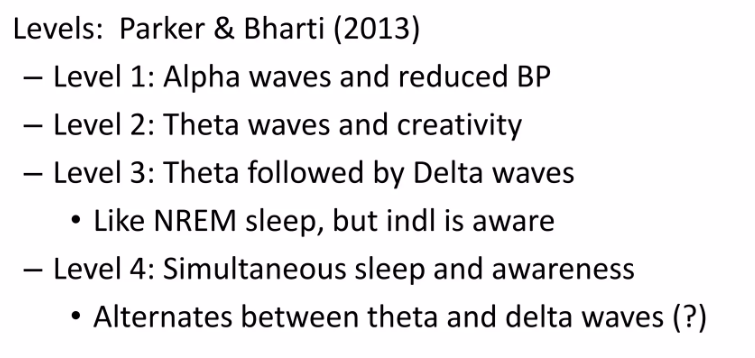
\includegraphics[width=0.8\linewidth,keepaspectratio]{yoganidra10}

        % \end{center}

    \begin{itemize}
        \item Level 1: Alpha waves and reduced BP
        \item Level 2: Theta waves and creativity
        \item Level 3: Theta followed by Delta waves: Like NREM sleep, but individual is aware
        \item Level 4: Simultaneous sleep and awareness: Alternates between theta and delta waves (?)
    \end{itemize}
	
		{\tiny (Ref: Yoga Nidra - Dr Amit Chail)}		

\end{frame}



%%%%%%%%%%%%%%%%%%%%%%%%%%%%%%%%%%%%%%%%%%%%%%%%%%%%%%%%%%%%%%%%%%%%%%%%%%%%%%%%%%
\begin{frame}[fragile]\frametitle{8 Stages of Yoganidra}
    \begin{enumerate}
        \item \textbf{Preparation (Shavasana)}: Deep breaths in Shavasana (शवासन).
        \item \textbf{Resolve (Sankalpa)}: Optional positive affirmation (संकल्प).
        \item \textbf{Body Awareness (Rotation)}: Relax body parts.
        \item \textbf{Breath Awareness}: Relaxation through breath.
        \item \textbf{Opposite Sensations}: Experience and release emotions.
        \item \textbf{Visualization}: Reach the subconscious with imagery.
        \item \textbf{Resolve (Sankalpa)}: Repeat the Sankalpa again.
        \item \textbf{Exiting}: Return awareness to external surroundings.
    \end{enumerate}
\end{frame}

%%%%%%%%%%%%%%%%%%%%%%%%%%%%%%%%%%%%%%%%%%%%%%%%%%%%%%%%%%%%%%%%%%%%%%%%%%%%%%%%%%
\begin{frame}[fragile]\frametitle{Key Instructions}
    \begin{itemize}
        \item No movement during Yoganidra.
        \item Stay awake, do not fall asleep.
        \item Do not think, just follow the instructions.
    \end{itemize}
\end{frame}


%%%%%%%%%%%%%%%%%%%%%%%%%%%%%%%%%%%%%%%%%%%%%%%%%%%%%%%%%%%%%%%%%%%%%%%%%%%%%%%%%%
\begin{frame}[fragile]\frametitle{The Koshas (कोश)}
    \begin{itemize}
        \item \textbf{Annamaya Kosha (अन्नमयकोश)} - Physical Body
        \item \textbf{Pranamaya Kosha (प्राणमयकोश)} - Energy Body
        \item \textbf{Manomaya Kosha (मनोमयकोश)} - Emotional Body
        \item \textbf{Vijnanamaya Kosha (विज्ञानमयकोश)} - Wisdom Body
        \item \textbf{Anandamaya Kosha (आनन्दमयकोश)} - Bliss Body
    \end{itemize}
\end{frame}

%%%%%%%%%%%%%%%%%%%%%%%%%%%%%%%%%%%%%%%%%%%%%%%%%%%%%%%%%%%%%%%%%%%%%%%%%%%%%%%%%%
\begin{frame}[fragile]\frametitle{Koshas in Yoganidra}
    
    \begin{itemize}
        \item Body Awareness (Rotation): \textbf{Annamayakosha (अन्नमयकोश) - Physical Body:} Focus on different body parts (right palm, right arm, legs, back, etc.).
        \item Breath Awareness: \textbf{Pranamayakosha (प्राणमयकोश) - Breath Awareness:} Reverse breath count from 27.
        \item Opposite Sensations: \textbf{Manomayakosha (मनोमयकोश) - Emotional Body:} Experience opposite sensations (hot/cold, wet/dry).
        \item Visualization: \textbf{Vijnanamayakosha (विज्ञानमयकोश) - Subconscious Visualization:} Visualize calming scenes like deserts, lakes, and waves.
    \end{itemize}
\end{frame}

%%%%%%%%%%%%%%%%%%%%%%%%%%%%%%%%%%%%%%%%%%%%%%%%%%%%%%%%%%%%%%%%%%%%%%%%%%%%%%%%%%
\begin{frame}[fragile]\frametitle{Tips for Practicing Yoganidra}
    \begin{itemize}
        \item Use simple and precise language in the script.
        \item Speak in a clear and even tone.
        \item Sit comfortably and be still during facilitation.
        \item Practice in a warm, comfortable space. Use props (pillows, blankets) to support the body.
        \item Remain still, but do not fall asleep.
    \end{itemize}
\end{frame}

%%%%%%%%%%%%%%%%%%%%%%%%%%%%%%%%%%%%%%%%%%%%%%%%%%%%%%%%%%%
\begin{frame}[fragile]\frametitle{Important Considerations}
    \begin{itemize}
        \item \textbf{Consult Healthcare Provider if:}
        \begin{itemize}
            \item Pregnant or recently post-partum
            \item Have serious medical conditions
            \item Experiencing severe mental health issues
        \end{itemize}
        \item \textbf{Practice Guidelines:}
        \begin{itemize}
            \item Avoid practice immediately after meals
            \item Ensure comfortable room temperature
            \item Practice at consistent times
            \item Stay awake during the practice
        \end{itemize}
    \end{itemize}
\end{frame}

%%%%%%%%%%%%%%%%%%%%%%%%%%%%%%%%%%%%%%%%%%%%%%%%%%%%%%%%%%%
\begin{frame}[fragile]\frametitle{Benefits of Yoganidra for the Mind and Body}
    \begin{itemize}
        \item Deep relaxation and mental reset.
        \item Allows reprogramming of habitual negative thoughts.
        \item Enhances self-awareness and reduces stress.
        \item Promotes clarity, relaxation, and mental fortitude.
    \end{itemize}
\end{frame}

%%%%%%%%%%%%%%%%%%%%%%%%%%%%%%%%%%%%%%%%%%%%%%%%%%%%%%%%%%%
\begin{frame}[fragile]\frametitle{Limitations of Yoganidra}
    \begin{itemize}
        \item Its a mental, psychological process, so no physical problems are solved
		\item Can not cure diseases like diabetics but the mental trauma associated with it
    \end{itemize}
\end{frame}

%%%%%%%%%%%%%%%%%%%%%%%%%%%%%%%%%%%%%%%%%%%%%%%%%%%%%%%%%%%
\begin{frame}[fragile]\frametitle{Limitations of Yoganidra}
    \begin{itemize}
	    \item \textbf{Only for Psychological problems:} 
			\begin{itemize}
				\item Its a mental, psychological process, so no physical problems are solved
				\item Can not cure diseases like diabetics but the mental trauma associated with it
			\end{itemize}
			
        \item \textbf{Requires Guidance:} 
            \begin{itemize}
                \item Proper guidance from a skilled teacher or accurate recordings is essential for effective practice.
                \item Self-practice without understanding may lead to superficial relaxation without achieving deeper benefits.
            \end{itemize}
        
        % \item \textbf{Misinterpretation as Sleep:}
            % \begin{itemize}
                % \item Yoganidra is often misunderstood as a sleep replacement, but it doesn’t fulfill the same physiological requirements.
                % \item The goal is conscious relaxation, not unconscious sleep.
            % \end{itemize}

        \item \textbf{Effectiveness Depends on Regularity:}
            \begin{itemize}
                \item Practicing sporadically may yield limited benefits; consistency is needed for noticeable mental and emotional transformation.
                \item Results can take time, requiring patience and dedication.
            \end{itemize}
        
        \item \textbf{Not a Substitute for Therapy:}
            \begin{itemize}
                \item While beneficial for stress and self-awareness, Yoganidra may not replace therapeutic interventions for serious psychological issues.
                \item It is best used as a complementary practice rather than a sole treatment for mental health concerns.
            \end{itemize}
        
        % \item \textbf{Physical and Mental Readiness:}
            % \begin{itemize}
                % \item May not be suitable for individuals who find it difficult to lie still or relax, or for those with acute physical discomfort.
                % \item Requires some degree of mental stability and readiness to confront subconscious material.
            % \end{itemize}
        
        % \item \textbf{Expectations vs. Reality:}
            % \begin{itemize}
                % \item High expectations for instant results can lead to disappointment; benefits tend to accumulate gradually.
                % \item Practitioners should approach it with an open and patient mindset for best outcomes.
            % \end{itemize}
    \end{itemize}
\end{frame}
